\documentclass{article}
\usepackage[utf8]{inputenc}
\usepackage[T2A]{fontenc}
\usepackage[utf8]{inputenc}
\usepackage{float}
%\usepackage[russian]{babel}
\usepackage[a4paper, left=10mm, right=10mm, top=20mm, bottom=20mm]{geometry}
\usepackage{natbib}
\usepackage{graphicx}
\usepackage{tabularx}
\usepackage{hyperref}

\title{PSD@CBM firmware description (draft, for internal use)}
\author{Finogeev Dmitry, INR RAS}





\begin{document}

\maketitle

Actual version of the document is avaliable at github:
\newline
\url{https://github.com/dfinogee/PSD-readout-manual/raw/main/PSD_readout_manual.pdf}



\tableofcontents

\newpage

\section{ADC data processing}
PSD\_data\_readout component receive data from all ADCs, process waveform and output data in GBT packets. Schematic of component is presented on fig.~\ref{fig:1}.

\begin{figure}[H]
	\centering 
	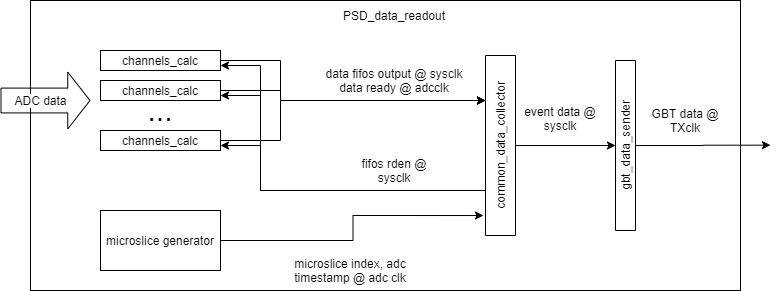
\includegraphics[width=0.8\textwidth]{ADC_readout.png}
	\caption{\label{fig:1} ADC data readout scheme}
\end{figure}




\subsection{Component channels\_calc}
Channel\_calc component scheme is presented on figure~\ref{fig:2}. ADC data inverted for negative signals, zero level and RMS are calculated and avaliable from slow control.


\begin{figure}[H]
	\centering 
	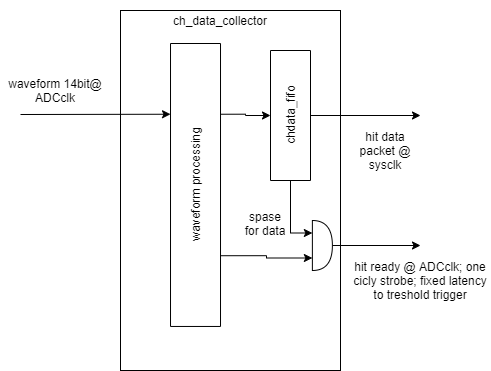
\includegraphics[width=1.0\textwidth]{ADC_event_collection.png}
	\caption{\label{fig:2} Channel data processing scheme}
\end{figure}


Strobe\_generator component forms waveform gate, start and stop signals by threshold crossing taking waveform length and offset parameters. Waveform data that are available from the start (zero level) are latched while strobe. Signal diagram of the component is presented on figure~\ref{fig:3} To reduce the probability of being triggered by a noise event, three neighboring points are compared with threshold. Central point is compared with the treshold value and two side points with half of threshold value.

Waveform offset parameter determine waveform position in gate, if it is 0, first point in waveform strobe is  the point above threshold (the third point compared to half of threshold value). Maximum offset value is 13. Latched baseline level is value before point above threshold.

If one channel in common trigger mask parameter cross threshold, common trigger is generated. All channels in common trigger output parameter take waveform similar to they has threshold crossing together.

\begin{figure}[H]
	\centering 
	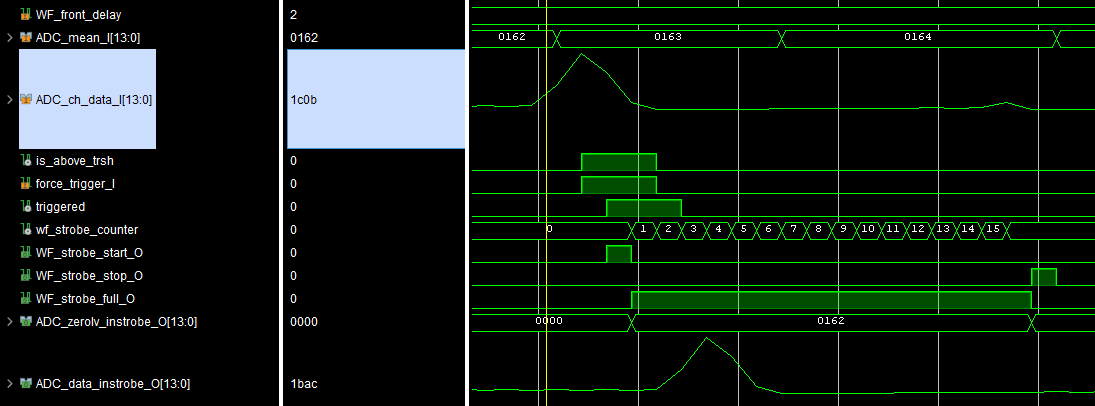
\includegraphics[width=0.8\textwidth]{wf_strobe_diag_sim.png}
	\caption{\label{fig:3} Signal waveform strobe (length 16, offset 3)}
\end{figure}


Ch\_data\_collector store waveform point in raw\_fifo by strobe signal and start waveform data (zero level) by start signal. When charge ready signal raised, charge and start data from header\_fifo stored in data\_fifo as hit packed header. This allow to upgrade charge calculation with fitting procedure and change calculation delay. In next cycle waveform points are read from raw\_fifo and (if sending wf points parameter is set on) stored as hit data in ch\_data\_fifo. After hit packet stored, ready signal raised or dropped signal in case fifo was full and hit packet was dropped. Ready and dropped signals are synchronous to threshold crossing and used for event ADC timestamp.  Signals diagramm of the component is presented on figure~\ref{fig:4}. The write size of ch\_data\_fifo should be equal to ceil(calculation\_delay / waveform\_lenght)*waveform\_lenght. The size of ch\_header\_fifo should be ceil(calculation\_delay / waveform\_lenght). Write rate for mentioned fifo is equal to read rate.
In case data-fifo is full while charge ready signal, hit is dropped and dropped-hits counter increased by 1. Dropped-hits counter is avaliable in channel status and reset after each register reading.

Readout-rate component allow to measure hit rate per channel. Waveform-start signals counted with 16bit counter and 70Hz rate. Each 70 Hz cycle, count is stored in 128 shift register. Rate-mean register store the summ of values stored in shift register. Two modes: low-rate and normal are available for rate reading. In normal mode for 16 bit status register available rate-mean[22 downto 7] and result is rate/70Hz. In low-rate mode (channel-low-rate-count bit) rate-mean[15 downto 0] avaliable for status register and result is rate/70*128Hz.

\begin{figure}[H]
	\centering 
	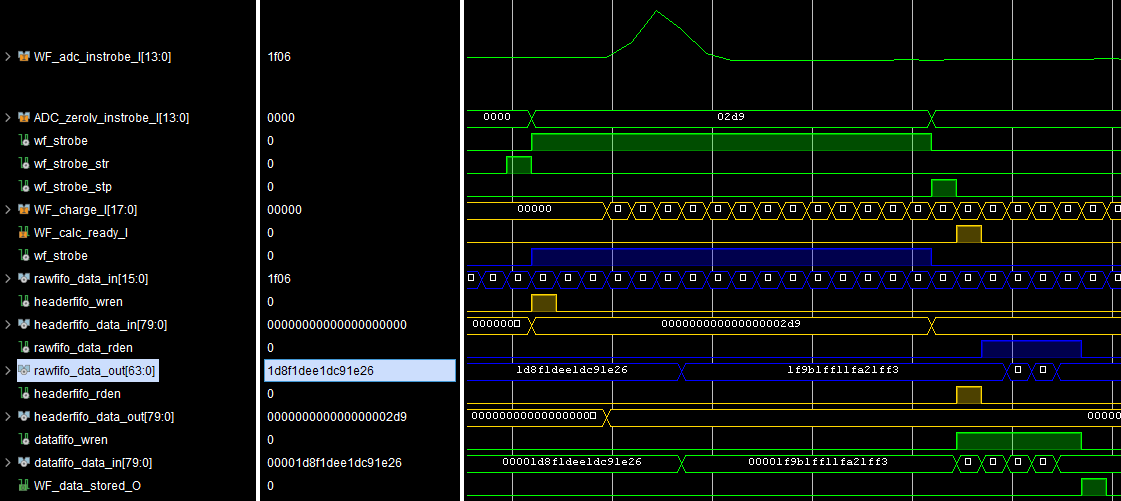
\includegraphics[width=1.0\textwidth]{ADC_ch_data_collector_wave.png}
	\caption{\label{fig:4} Channel data collecting signals}
\end{figure}

Signals could be processed one after another without dead time. If next adc point after waveform gate is higher than threshold, new signal gate is formed. Signal time is next adc cycle after first gate, not is real time of second waveform threshold crossing. Signal diagram for such case is presented on figure~\ref{fig:5}.


\begin{figure}[H]
	\centering 
	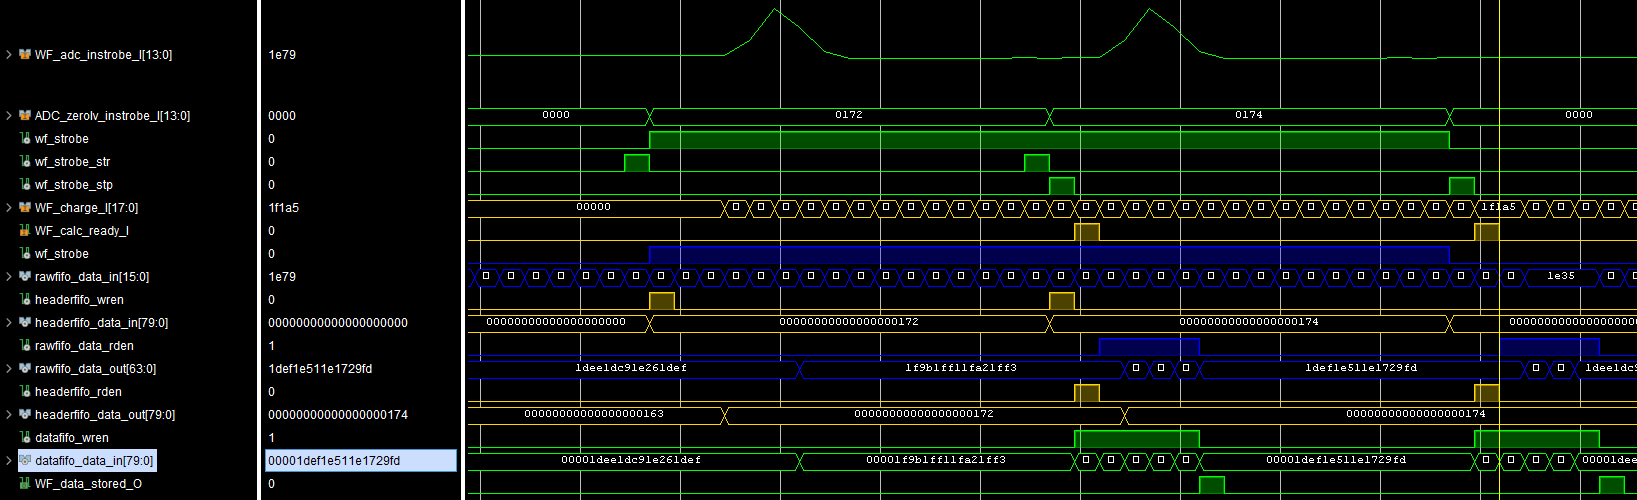
\includegraphics[width=1.0\textwidth]{ADC_ch_data_collector_wave_pileup.png}
	\caption{\label{fig:5} Channel data collecting signals}
\end{figure}

\subsection{Component common\_data\_collector}
Each channel generate single strobe with fixed latency to threshold crossing indicating waveform measurement. 32 bit strobe word is stored to data\_wf\_calc\_fifo with mc index and ADC timestamp. FSM read stored strobes and collect data from fired channels storing outputs to common\_data\_fifo, each event header word with timing and data size info stored in common\_header\_fifo. Shematic represented on figure ~\ref{fig:3}.

\begin{figure}[H]
	\centering 
	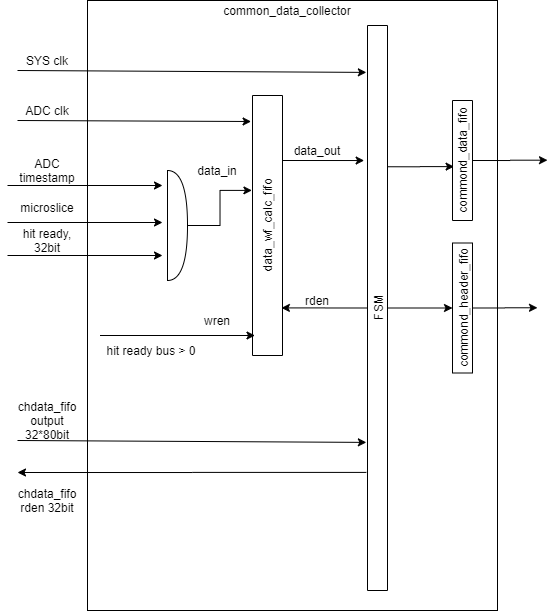
\includegraphics[width=0.5\textwidth]{ADC_common_event_collection.png}
	\caption{\label{fig:6} Data collecting scheme from all channels fifos}
\end{figure}


FSM is switched from wait to start state when data\_wf\_calc\_fifo\_isempty became '0' and fifo output is latched. Priority encoder show next fired channel from strobe and data collected from fired channel to common\_data\_fifo with hit\_packet\_iterator. Input to priory encoder is shifted to bit after fired channel when iterator reach last fired channel. Priority encoder could be equal or less than 32 bit. Simulation outputs presented on figure ~\ref{fig:4}.

\begin{figure}[H]
	\centering 
	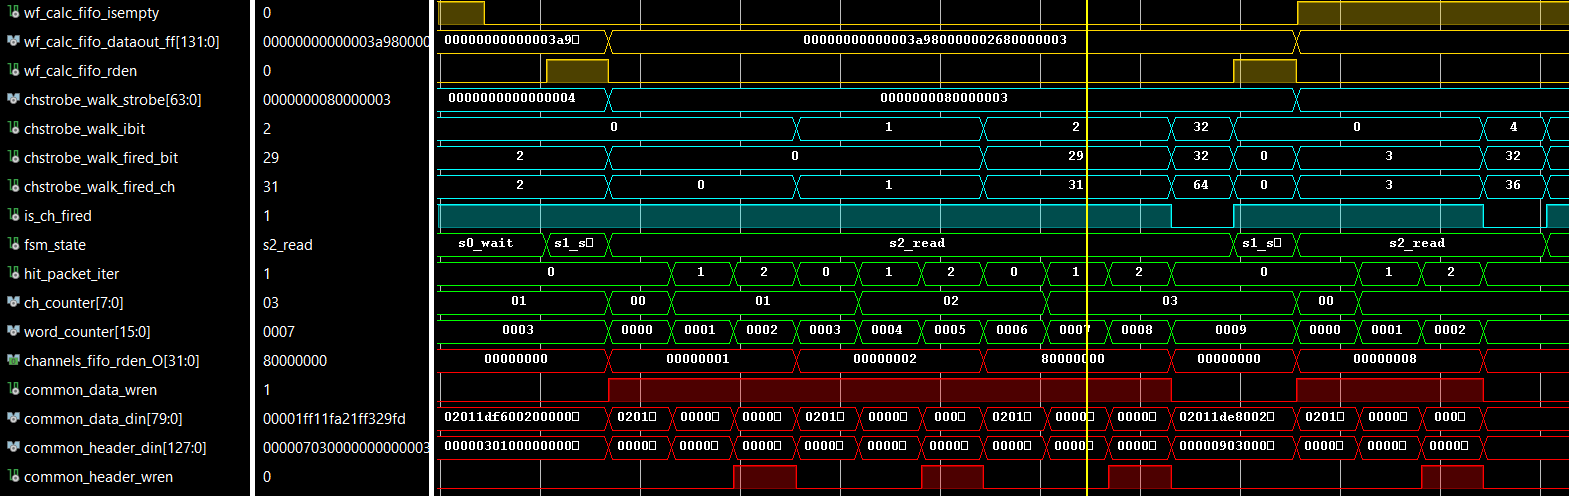
\includegraphics[width=1.0\textwidth]{ADC_common_data_collector_wave.png}
	\caption{\label{fig:7} Data collecting signal from all channels fifos}
\end{figure}

Collecting data from all channels takes two additional FSM cycle. Mean hit rate per channel in case all channels fired is SYSCKL / total channels + 2 cycle / packet length. Test beam: 80MHz / 12 / 5 = 1.3MHz. Final setup: 120 (240) / 32 / 1 = 3.5 (7) MHz.


\subsection{Component GBT\_data\_sender}

Data stored in common\_data\_fifo in component common\_data\_collector are read by system clock with writing rate. Event and microslice headers are formed by data from common\_header\_fifo. Built GBT data packets are stored in gbt\_data\_fifo and read by GBT TX clock. Signal diagram is presented on figure~\ref{fig:8}. 


\begin{figure}[H]
	\centering 
	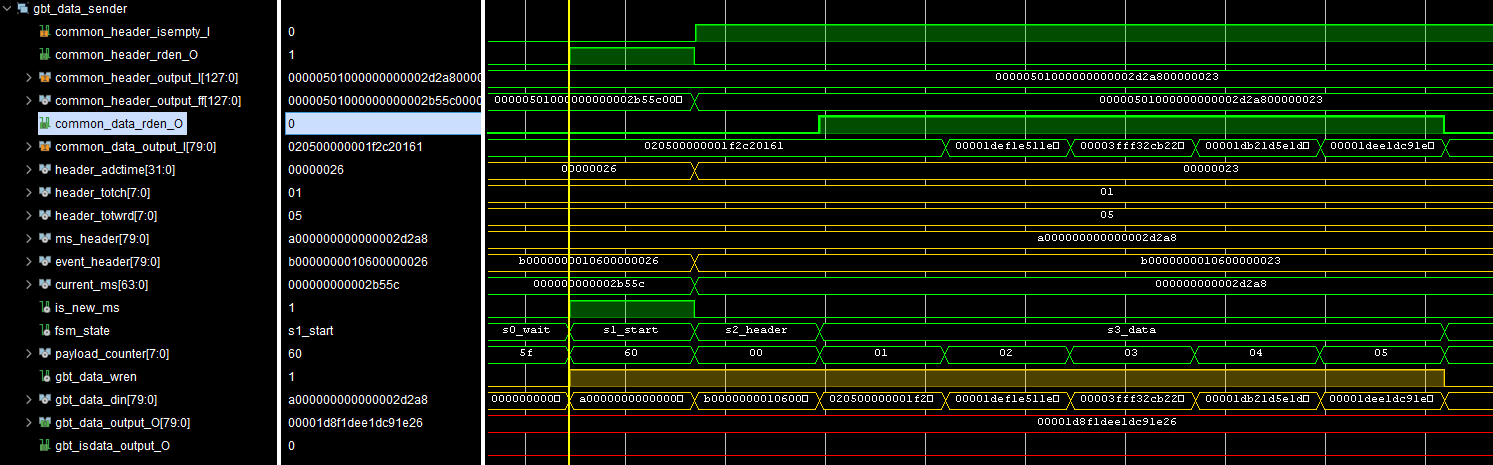
\includegraphics[width=1.0\textwidth]{GBT_sender_wave.png}
	\caption{\label{fig:8} Channel data collecting signals}
\end{figure}



Data rate limit is 80bit X 40MHz = 0.4 GB/s(GBT). Hit rate limit per channel (without microslice word) is 40MHz / 33 (packet length) = 1,2 MHz in case all channels are fired. The rate could be increased to  2.4 MHz hits per channel in case all 32 channels are fired. If one hit data will be less than 40bit event packet will contain 17 GBT words.

GBT packet format is presented on tables: ~\ref{tab1}, ~\ref{tab2}, ~\ref{tab3}





\begin{table}[H]
\centering
\begin{tabular}{| l | l | l | l | l | l | l | l | l |}
\hline
word type & 79 .. 76 & 75 .. 72 & 71 .. 64 & 63 .. 48 & 47 .. 40 & 39 .. 32 & 31 .. 16 & 15 .. 0 \\ \hline
ms header & 0xA & \multicolumn{2}{c|}{0x0}  & \multicolumn{5}{c|}{ms index} \\ \hline
event header & 0xB & ADC idx** & \multicolumn{2}{c|}{0x0} & n fired channels & words in packet * & \multicolumn{2}{c|}{adc time} \\ \hline
hit header & \multicolumn{8}{c|}{hit header (tab.~\ref{tab1})} \\ \hline
hit data & \multicolumn{8}{c|}{hit data (tab.~\ref{tab2})} \\ \hline
hit data & \multicolumn{8}{c|}{hit data (tab.~\ref{tab2})} \\ \hline
hit data & \multicolumn{8}{c|}{hit data (tab.~\ref{tab2})} \\ \hline
hit data & \multicolumn{8}{c|}{hit data (tab.~\ref{tab2})} \\ \hline
  & \multicolumn{8}{c|}{ ... } \\ \hline

event header & 0xB & ADC idx** & \multicolumn{2}{c|}{0x0} & n fired channels & words in packet * & \multicolumn{2}{c|}{adc time} \\ \hline
  & \multicolumn{7}{c|}{ ... } \\ \hline

\end{tabular}
\caption{GBT data format. [* number of GBT words in event packet: event header + all hit packets] [** ADC board index] \label{tab1}}
\end{table}

\begin{table}[H]
\centering
\begin{tabular}{| l | l | l | l | l | l |}
\hline
word & 79 .. 72 & 71 .. 64 & 63 .. 36 & 35 .. 16 & 15 .. 0 \\ \hline
1 & channel &words in packet *& 0x0 & signal charge & waveform zero level \\ \hline
\end{tabular}
\caption{hit packet header. [* total GBT words in hit packet: header + data words]\label{tab2}}
\end{table}

\begin{table}[H]
\centering
\begin{tabular}{| l | l | l | l | l | l |}
\hline
word & 79 .. 64 & 63 .. 48 & 47 .. 32 & 31 .. 16 & 15 .. 0 \\ \hline
1 & 0x0 & waveform point n & waveform point n+1 & waveform point n+2 & waveform point n+3 \\ \hline
\end{tabular}
\caption{hit packet data word.\label{tab3}}
\end{table}


\section{ADC control}
\subsection{Control registers}

To avoid configuration corruption while GBT link fail, register 31 is reserved for lock key word. Control registers are available for writing if register 31 is 0xafafafaf. Register 31 is always open for writing.

\begin{table}[H]
\centering
\begin{tabular}{| l | l | l | l | l | l | l | l | l | l | l |}
\hline
addr & 31 .. 30 & 29 .. 28 & 27 .. 24 & 23 .. 20 & 19 .. 16 & 15 .. 14 & 13 .. 12 & 11 .. 8 & 7 .. 4 & 3 .. 0 \\ \hline
0 & 0x0 & \multicolumn{4}{c|}{threshold ch1} & 0x0 & \multicolumn{4}{c|}{threshold ch0} \\ \hline
1 & 0x0 & \multicolumn{4}{c|}{threshold ch3} & 0x0 & \multicolumn{4}{c|}{threshold ch2} \\ \hline
2 & 0x0 & \multicolumn{4}{c|}{threshold ch5} & 0x0 & \multicolumn{4}{c|}{threshold ch4} \\ \hline
3 & 0x0 & \multicolumn{4}{c|}{threshold ch7} & 0x0 & \multicolumn{4}{c|}{threshold ch6} \\ \hline
4 & 0x0 & \multicolumn{4}{c|}{threshold ch9} & 0x0 & \multicolumn{4}{c|}{threshold ch8} \\ \hline
5 & 0x0 & \multicolumn{4}{c|}{threshold ch11} & 0x0 & \multicolumn{4}{c|}{threshold ch10} \\ \hline
6 & 0x0 & \multicolumn{4}{c|}{threshold ch13} & 0x0 & \multicolumn{4}{c|}{threshold ch12} \\ \hline
7 & 0x0 & \multicolumn{4}{c|}{threshold ch15} & 0x0 & \multicolumn{4}{c|}{threshold ch14} \\ \hline
8 & 0x0 & \multicolumn{4}{c|}{threshold ch17} & 0x0 & \multicolumn{4}{c|}{threshold ch16} \\ \hline
9 & 0x0 & \multicolumn{4}{c|}{threshold ch19} & 0x0 & \multicolumn{4}{c|}{threshold ch18} \\ \hline
10 & 0x0 & \multicolumn{4}{c|}{threshold ch21} & 0x0 & \multicolumn{4}{c|}{threshold ch20} \\ \hline
11 & 0x0 & \multicolumn{4}{c|}{threshold ch23} & 0x0 & \multicolumn{4}{c|}{threshold ch22} \\ \hline
12 & 0x0 & \multicolumn{4}{c|}{threshold ch25} & 0x0 & \multicolumn{4}{c|}{threshold ch24} \\ \hline
13 & 0x0 & \multicolumn{4}{c|}{threshold ch27} & 0x0 & \multicolumn{4}{c|}{threshold ch26} \\ \hline
14 & 0x0 & \multicolumn{4}{c|}{threshold ch29} & 0x0 & \multicolumn{4}{c|}{threshold ch28} \\ \hline
15 & 0x0 & \multicolumn{4}{c|}{threshold ch31} & 0x0 & \multicolumn{4}{c|}{threshold ch30} \\ \hline
\end{tabular}
\caption{ADC channels threshold control.\label{tab4}}
\end{table}

\begin{table}[H]
\centering
\begin{tabular}{| l | l | l | l | l | l | l | l | l |}
\hline
addr & 31 .. 28 & 27 .. 24 & 23 .. 20 & 19 .. 16 & 15 .. 12 & 11 .. 8 & 7 .. 4 & 3 .. 0 \\ \hline
16 & \multicolumn{2}{c|}{0x0} & \multicolumn{2}{c|}{status ch sel} & waveform length 0..3 [(reg+1)*4] & strobe offset 0..12 & \multicolumn{2}{c|}{control bits} \\ \hline
17 & \multicolumn{8}{c|}{negative channel mask ibit = ich} \\ \hline
18 & \multicolumn{8}{c|}{I2C HV bus} \\ \hline
19 & \multicolumn{8}{c|}{microslice gen counter@25ns} \\ \hline
20 & \multicolumn{8}{c|}{microslice period} \\ \hline
21 & \multicolumn{8}{c|}{common trigger mask *} \\ \hline
22 & \multicolumn{8}{c|}{common trigger output **} \\ \hline
\end{tabular}
\caption{ADC readout control. [* channels set generates common trigger] [** triggered channels set]\label{tab5}}
\end{table}

\begin{table}[H]
\centering
\begin{tabular}{| l | l |}
\hline
bit & description \\ \hline
0 & send waveform \\ \hline
1 & ms gen standalone \\ \hline
2 & readout fsm reset \\ \hline
3 & errors reset \\ \hline
4 & channel low rate count \\ \hline
\end{tabular}
\caption{Control bits\label{tab6}}
\end{table}


\begin{table}[H]
\centering
\begin{tabular}{| l | l | l | l | l | l | l | l | l |}
\hline
addr & 31 .. 18 & 17 .. 17 & 16 .. 16 & 15 .. 8 & 7 .. 7 & 6 .. 0 \\ \hline
18 & 0x0 & WR & ENA & DATA & 0x0 & ADDR \\ \hline
\end{tabular}
\caption{HV control via I2C.\label{tab7}}
\end{table}


\subsection{Status registers}

Status registers map is presented on table \ref{tab8}. 

\begin{table}[H]
\centering
\begin{tabular}{| l | l | l | l | l | l | l | l | l | l | l |}
\hline
addr & 31 .. 30 & 29 .. 28 & 27 .. 24 & 23 .. 20 & 19 .. 16 & 15 .. 14 & 13 .. 12 & 11 .. 8 & 7 .. 4 & 3 .. 0 \\ \hline
0 & \multicolumn{10}{c|}{microslice index 31 .. 0}\\ \hline
1 & \multicolumn{10}{c|}{microslice index 63 .. 32}\\ \hline
2 & \multicolumn{10}{c|}{ADC time}\\ \hline
3 & \multicolumn{5}{c|}{RX wrclk err cnt} & \multicolumn{5}{c|}{RX err frclk cnt} \\ \hline
4 & \multicolumn{5}{c|}{RX err detect cnt} & \multicolumn{5}{c|}{I2C HV bus}\\ \hline
5 & \multicolumn{8}{c|}{0x0} & \multicolumn{2}{c|}{temp} \\ \hline
6 & \multicolumn{5}{c|}{sel. channel baseline rms} & \multicolumn{5}{c|}{sel. channel baseline}\\ \hline
7 & \multicolumn{5}{c|}{sel. channel dropped hits} & \multicolumn{5}{c|}{sel. channel hit rate}\\ \hline
\end{tabular}
\caption{ADC channels threshold control.\label{tab8}}
\end{table}

\begin{table}[H]
\centering
\begin{tabular}{| l | l | l | l | l | l | l | l | l |}
\hline
addr & 15 .. 10 & 9 .. 9 & 8 .. 8 & 7 .. 0 \\ \hline
4 & 0x0 & error ack & busy & DATA \\ \hline
\end{tabular}
\caption{HV status via I2C.\label{tab9}}
\end{table}

Status registers comments:
\begin{itemize}
\item RX err detect cnt - counter@RXclk of RX error detected bit.

\item RX err frclk cnt - counter@RXclk of state when frame clock is not ready.

\item RX wrclk err cnt - counter@RXclk of state when word clock is not ready.


\end{itemize}


\section{CRI modules}

\subsection{PSD CRI data sorting}

\begin{figure}[H]
	\centering 
	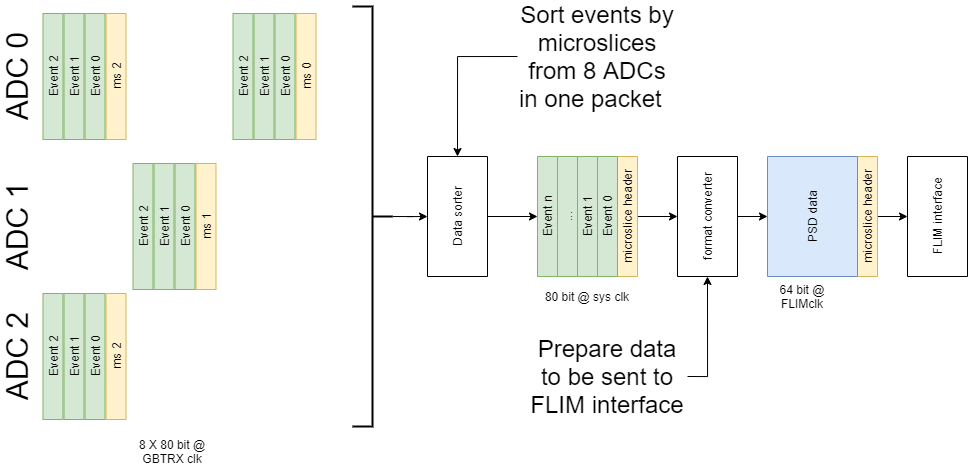
\includegraphics[width=1.0\textwidth]{CRI_data_sort.png}
	\caption{\label{fig:11} PSD data processing in CRI}
\end{figure}


\subsection{ADC GBT emulator}

ADC GBT emulator generate GBT ADC packets filling hit packages with continuous hit counter. Parameters are:

\begin{itemize}
\item ms\_index - current microslice index @GBTclk to generate ms headers.


\item  event\_rate is number of GBT clock cycles between packets (from start to start). If previous packet was not sent, and is time to generate new one, new one skipped.

\item nch\_in\_even - number of hits per event 1 ... 32. Emulate fired channels.

\item hit\_packet\_len - number of hit packet words, including hit header 1 ... 5.

\end{itemize}

Emulator FSM is based on three counters, signals diagram is presented on figure \ref{fig:9}; generated data format is presented on figure \ref{tab8}.

\begin{figure}[H]
	\centering 
	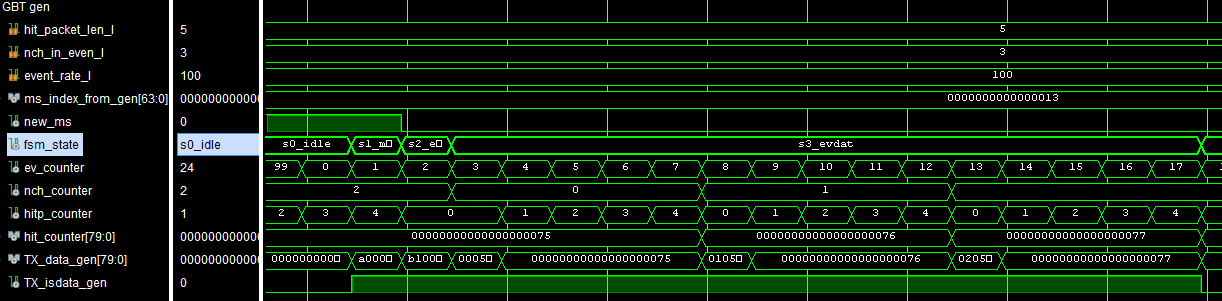
\includegraphics[width=1.0\textwidth]{ADC_GBT_emu_waves.png}
	\caption{\label{fig:9} ADC GBT emulator signals}
\end{figure}

\begin{table}[H]
\centering
\begin{tabular}{| l | l | l | l | l | l | l | l | l |}
\hline
word type & 79 .. 76 & 75 .. 72 & 71 .. 64 & 63 .. 48 & 47 .. 40 & 39 .. 32 & 31 .. 16 & 15 .. 0 \\ \hline
ms header & 0xA & \multicolumn{2}{c|}{0x0}  & \multicolumn{5}{c|}{ms index} \\ \hline
event header & 0xB & ADC idx** & \multicolumn{2}{c|}{0x0} & n hits & packet len * & \multicolumn{2}{c|}{0x0} \\ \hline
hit header & \multicolumn{2}{c|}{hit number} & words in hit packet *** & \multicolumn{5}{c|}{ms index} \\ \hline
hit data & \multicolumn{8}{c|}{hit counter [79 ..0]} \\ \hline
hit data & \multicolumn{8}{c|}{hit counter [79 ..0]} \\ \hline
hit data & \multicolumn{8}{c|}{hit counter [79 ..0]} \\ \hline
hit data & \multicolumn{8}{c|}{hit counter [79 ..0]} \\ \hline
  & \multicolumn{8}{c|}{ ... } \\ \hline

event header & 0xB & ADC idx** & \multicolumn{2}{c|}{0x0} & n hits & packet len * & \multicolumn{2}{c|}{0x0} \\ \hline
  & \multicolumn{7}{c|}{ ... } \\ \hline

\end{tabular}
\caption{GBT data format. [* number of GBT words in event packet: event header + all hit packets] [** ADC board index] [*** total words in hit packet, including hit header]\label{tab10}}
\end{table}


\subsection{ADC GBT reader}
ADC GBT reader reads GBT packets from one GBT link and store its to fifo event\_fifo. With last packet data word header word pushed to separate fifo header\_ fifo with packet lenght and microslice index. Event packet skipped when one of fifos is full. After reset fsm starts wait microslice header. Packets reads according to size in header and fsm wait next packet or microslice header. If next word after packet is neither ms or packet header, fsm starts wait ms header. Data drop info state is not implemented yet. Signal diagram is presented on figure \ref{fig:11}. 

\begin{figure}[H]
	\centering 
	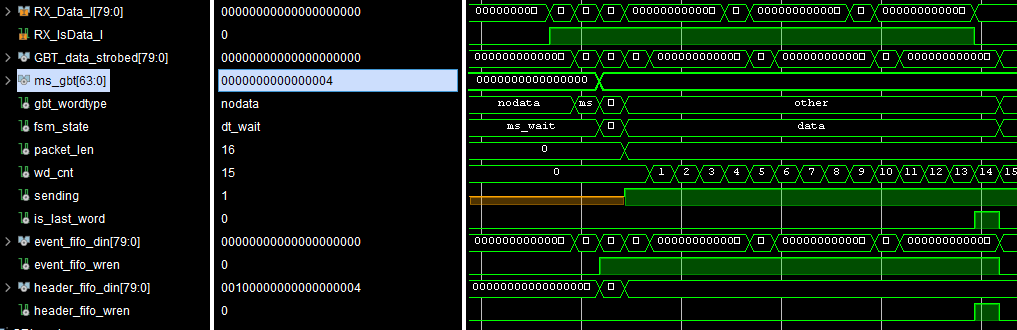
\includegraphics[width=1.0\textwidth]{ADC_GBT_reader_wave.png}
	\caption{\label{fig:11} ADC GBT packets reader}
\end{figure}

\subsection{GBT Data Sorter component}
Components header\_fifo and event\_fifo from adc-gbt-readers for all gbt links are connected to gbt-data-sorter component. Each new microslice value collected in ms-fifo. FSM switch thought all gbt links and read all one by one links with microslice less or equal to current microslice. Data for links with equal microslice to current-ms output from the sorter, for links with less microslice data is dropped. When all links have ms higher than current ms or are empty means that all data for current microslie are read. Such condition starts counter to wait data from all links. Then counter reach value 127, FSM swithced to next-ms state. Next microslice readed from fifo and header with new ms value sent to output stream. Signal diagram presented on figure \ref{fig:10} Output data represent combined GBT packets from all GBT link. All events from GBT links for one microslice follows one after another. Data for different microslices divided by microslice header with format 0xDAF0 + microslice (64bit). 


\begin{figure}[H]
	\centering 
	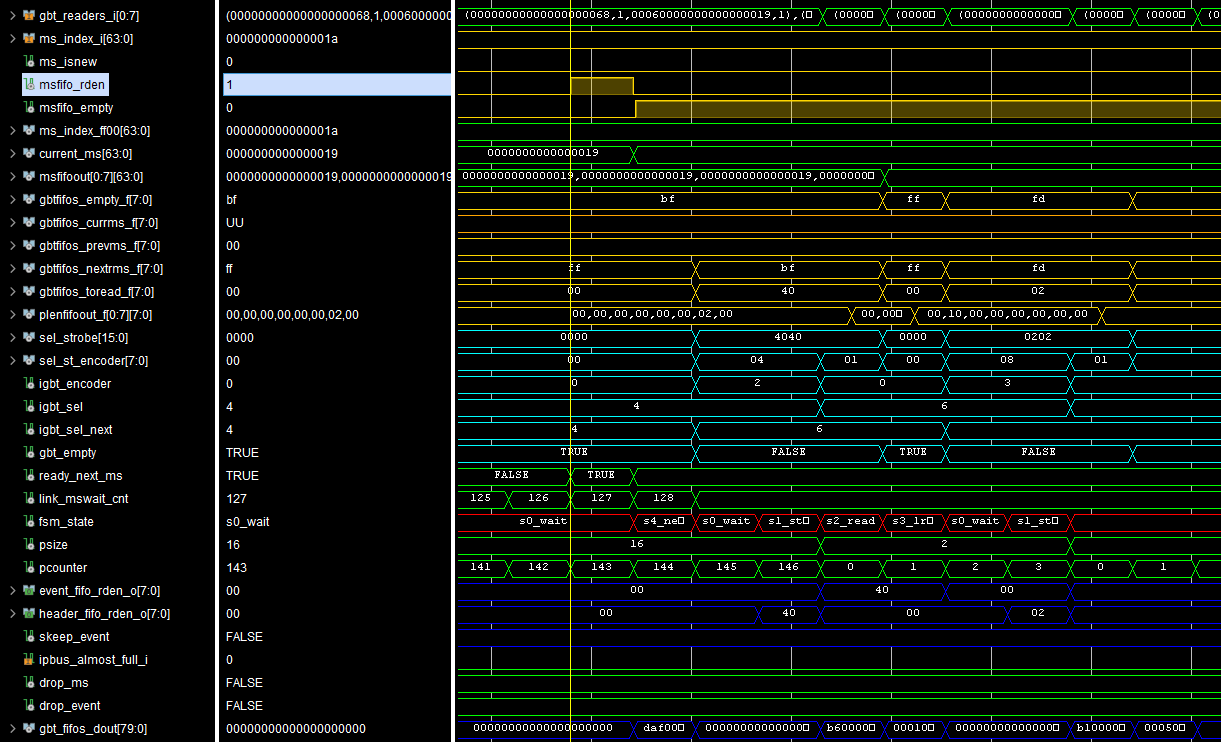
\includegraphics[width=1.0\textwidth]{gbt-sorter-waves.png}
	\caption{\label{fig:10} gbt-data-sorter signals diagram: mew ms read and event sent from one link }
\end{figure}


\subsection{IPbus face component}
IPbus-face-component read data stream from gbt-data-sorter and resize data to width 32 bit. Data stream from gbt-data-sorter stored in fifo-ipbus-face with 80bit write width and 160 read width. Output 160bit word divided in 5 32bit words. Each IPbus read cycle counter 0..4 increased by one, fifo-ipbus-face readed when counter equal 4 and ipbus-read signal is up. While reading empty fifo-ipbus-face all bits are '1'. Signals diagram is presented on figure \ref{fig:11}.

\begin{figure}[H]
	\centering 
	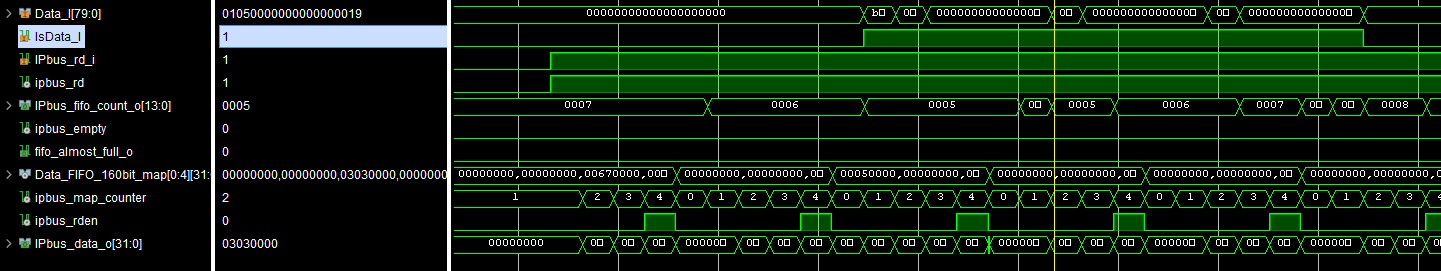
\includegraphics[width=1.0\textwidth]{ipbus-face-waves.png}
	\caption{\label{fig:11} IPbus-face signals diagram }
\end{figure}


\subsection{Evaluation Board for readout}

Kintex Evaluation board include CRI data processing module and use IPbus-face module for readout. Real GBT link is connected to 0 link, other links can receive data from emulators. Simple microslice generator is used to provide ms to gbt-data-sorter and to ADC board. Tables \ref{tab11} and \ref{tab13} present control and status registers map. GBT slow control and IPbus readout ported via dedicated addresses prioritized to status and control registers (could replace status and control registers), shown in table \ref{tab15} 



\begin{table}[H]
\centering
\begin{tabular}{| l | l | l | l | l | l | l | l | l |}
\hline
addr & 31 .. 28 & 27 .. 24 & 23 .. 20 & 19 .. 16 & 15 .. 12 & 11 .. 8 & 7 .. 4 & 3 .. 0 \\ \hline
0 & \multicolumn{6}{c|}{0x0}  & \multicolumn{2}{c|}{control word} \\ \hline
1 & \multicolumn{8}{c|}{microslice gen counter@25ns}  \\ \hline
2 & \multicolumn{8}{c|}{microslice period}  \\ \hline
\end{tabular}
\caption{Evaluation board control registers.\label{tab11}}
\end{table}

\begin{table}[H]
\centering
\begin{tabular}{| l | l |}
\hline
bit & description \\ \hline
0 & data processing reset \\ \hline

\end{tabular}
\caption{Control word bits\label{tab12}}
\end{table}


\begin{table}[H]
\centering
\begin{tabular}{| l | l | l | l | l | l | l | l | l |}
\hline
addr & 31 .. 28 & 27 .. 24 & 23 .. 20 & 19 .. 16 & 15 .. 12 & 11 .. 8 & 7 .. 4 & 3 .. 0 \\ \hline
0 & \multicolumn{4}{c|}{0x0}  & \multicolumn{4}{c|}{GBT status} \\ \hline

\end{tabular}
\caption{Evaluation board status registers.\label{tab13}}
\end{table}

\begin{table}[H]
\centering
\begin{tabular}{| l | l |}
\hline
bit & description \\ \hline
0 & MGT phalin cpll lock \\ \hline
1 & RX word clock ready \\ \hline
2 & RX frame clock ready \\ \hline
3 & MGT link ready \\ \hline
4 & TX reset done \\ \hline
5 & TX FSM reset done \\ \hline
6 & RX ready \\ \hline
7 & RX error detected \\ \hline
8 & RX error latched \\ \hline
\end{tabular}
\caption{GBT status bits\label{tab14}}
\end{table}


\begin{table}[H]
\centering
\begin{tabular}{| l | l | l |}
\hline
bit & description \\ \hline
64+2 & GBT slow cntrl wr & WR \\ \hline
64+3 & GBT slow cntrl rd & RD \\ \hline
64+4 & IPbus readout fifo count & RD \\ \hline
64+5 & IPbus readout fifo data & RD \\ \hline
\end{tabular}
\caption{Dedicated bus registers\label{tab15}}
\end{table}


\end{document}

